%! Author = Omar Iskandarani
%! Title = Swirl String Theory (SST) Canonical Fluid Reformulation of Relativity and Quantum Structure
%! Date = Oct, 2025
%! Affiliation = Independent Researcher, Groningen, The Netherlands
%! License = © 2025 Omar Iskandarani. All rights reserved. This manuscript is made available for academic reading and citation only. No republication, redistribution, or derivative works are permitted without explicit written permission from the author. Contact: info@omariskandarani.com
%! ORCID = 0009-0006-1686-3961
%! DOI = 10.5281/zenodo.xxxxx

\newcommand{\paperversion}{\textbf{v1.0.0}}
\newcommand{\papertitle}{\textbf{Swirl--String Theory:\A Canonical Fluid Reformulation of Relativity and Quantum Structure}}
\newcommand{\paperdoi}{10.5281/zenodo.xxxx}

%========================================================================================
% PACKAGES AND DOCUMENT CONFIGURATION
%========================================================================================
\documentclass[10pt,reprint,aps,onecolumn,nofootinbib]{revtex4-2}

\usepackage[utf8]{inputenc}
\usepackage[T1]{fontenc}
\usepackage[margin=2.3cm]{geometry}
\usepackage{amsmath,amssymb,amsfonts,bm}
\usepackage{adjustbox}
\usepackage{tikz}
\usetikzlibrary{matrix,positioning}
\usetikzlibrary{arrows.meta,positioning,calc,fit,decorations.pathmorphing}
\usetikzlibrary{matrix, positioning, fit, backgrounds}
\usepackage{siunitx} % optional; comment out if you prefer raw fractions
\sisetup{per-mode=symbol,detect-weight=true,detect-family=true}
\usepackage{hyperref}


% ===============================
% Macros (canonicalized)
% ===============================

% swirl arrows (context-aware)
\newcommand{\swirlarrow}{%
    \mathchoice{\mkern-2mu\scriptstyle\boldsymbol{\circlearrowleft}}%
    {\mkern-2mu\scriptscriptstyle\boldsymbol{\circlearrowleft}}%
}
\newcommand{\swirlarrowcw}{%
    \mathchoice{\mkern-2mu\scriptstyle\boldsymbol{\circlearrowright}}%
    {\mkern-2mu\scriptscriptstyle\boldsymbol{\circlearrowright}}%
}

% Canonical symbols
\newcommand{\vswirl}{\mathbf{v}_{\swirlarrow}}
\newcommand{\vswirlcw}{\mathbf{v}_{\swirlarrowcw}}
\newcommand{\SwirlClock}{S_{(t)}^{\swirlarrow}}
\newcommand{\SwirlClockcw}{S_{(t)}^{\swirlarrowcw}}
% sector/label style for scalar “max force”
\newcommand{\Fmaxswirl}{F^{\max}_{\mkern-1mu\scriptscriptstyle\boldsymbol{\circlearrowleft}}}
\newcommand{\Fmaxswirlcw}{F^{\max}_{\mkern-1mu\scriptscriptstyle\boldsymbol{\circlearrowright}}}
\newcommand{\FmaxEM}{F^{\max}_{\mathrm{EM}}}

\newcommand{\omegas}{\boldsymbol{\omega}_{\swirlarrow}}  % swirl vorticity
\newcommand{\vscore}{v_{\swirlarrow}}                    % shorthand: |v_swirl| at r=r_c
\newcommand{\vnorm}{\lVert \vswirl \rVert}               % swirl speed magnitude
\newcommand{\rhof}{\rho_{\!f}}                           % effective fluid density
\newcommand{\rhoE}{\rho_{\!E}}                           % swirl energy density
\newcommand{\rhom}{\rho_{\!m}}                           % mass-equivalent density
\newcommand{\rc}{r_c}                                    % string core radius (swirl string radius)
\newcommand{\Lam}{\Lambda}                               % Swirl Coulomb constant
\newcommand{\Om}{\Omega_{\swirlarrow}}                   % swirl angular frequency profile
% --- Minimal macro prelude (safe, local) ---
\providecommand{\rc}{r_c}
\newcommand{\omegaVec}{\boldsymbol{\omega}}
\newcommand{\rhoF}{\rho_{\!f}}     % effective fluid density
\newcommand{\rhoM}{\rho_{\!m}}     % mass-equivalent density
\newcommand{\OmegaCore}{\Omega_{\mathrm{core}}}
\newcommand{\bg}{\mathrm{bg}}
\newcommand{\core}{\mathrm{core}}
\newcommand{\Vol}{\operatorname{Vol}}   % now \Vol_{\!\mathbb{H}}(K) works

% ===============================
% Policy: the golden constant is only allowed via hyperbolic functions.
\newcommand{\xig}{\operatorname{asinh}\!\left(\tfrac{1}{2}\right)}
\newcommand{\phig}{\exp(\xig)}
\newcommand{\phialg}{\bigl(1+\sqrt{5}\bigr)/2}
\newcommand{\xigold}{\tfrac{3}{2}\,\xig}
\newcommand{\GoldenDeclare}{%
    \textbf{Golden (hyperbolic)}:\ \(\ln\phi=\xig\), hence \(\phi=\phig\).
    \ \emph{(Equivalently, \(\phi=\phialg\); the algebraic form is derivative.)}%
}

\newcommand{\vswirltext}{\mathbf{v}_{\mathrm{swirl}}}

\begin{document}
\title{\papertitle}
\author{Omar Iskandarani}
\affiliation{Independent Researcher, Groningen, The Netherlands}
\thanks{ORCID: 0009-0006-1686-3961, DOI: \paperdoi}
\date{\today}

\begin{abstract}

We present \emph{Swirl--String Theory} (SST), a fluid-topological framework that reinterprets relativity and quantum phenomena via a single incompressible medium. In SST, matter and radiation are modeled as quantized vortex loops (\emph{swirl strings}) in a universal, non-dissipative condensate. The theory posits that classical gravity emerges as a collective pressure effect of these vortices rather than fundamental spacetime curvature, and that local \emph{swirl flows} induce time dilation analogous to relativistic kinematics. We develop the formal field-theoretic Lagrangian for this medium, showing how a preferred foliation and topological quantization yield a discrete particle spectrum: quantum numbers (mass, charge, spin) correspond to topological invariants of knot-like vortex excitations. A modified Faraday's law is derived, unifying electromagnetic induction with rotating-frame effects by predicting that time-varying swirl string density generates an electromotive force. We also describe how SST accounts for wave--particle duality through dual phase (un-knotted vs. knotted) states of vortex loops, with quantum measurement corresponding to topological transitions. Several experimental tests are proposed to falsify or support SST, including quantized electromagnetic impulses from vortex reconnection events, attosecond-scale chirality-dependent time delays in photoemission, and interference degradation due to finite vacuum vorticity. We compare SST with established frameworks---from Kelvin's vortex atom hypothesis to emergent gravity and analogue fluid models---highlighting how SST recovers known limits (Newtonian gravity, Maxwell electrodynamics, quantum wave behavior) while providing novel, quantifiable predictions. All equations are given in SI units with attention to dimensional consistency. The result is a self-contained canonical reformulation that bridges classical and quantum physics through fluid-like continuum mechanics.

\emph{Keywords:} vortex dynamics; topological fluid; quantum topology; emergent gauge theory; time dilation; wavefunction collapse
\end{abstract}
\maketitle



\section{Introduction}
    \label{sec:intro}
    Reconciling General Relativity (GR) with Quantum Mechanics (QM) remains difficult because GR treats spacetime as dynamical and curved, whereas quantum field theories (QFT) typically operate on a fixed background. Swirl–String Theory (SST) approaches this tension by positing a unified substrate: a flat-space, incompressible condensate that supports and constrains all excitations.

    \subsection*{Motivation: Recasting the GR–QM Mismatch}
        The long–standing mismatch between the Standard Model (SM) and GR suggests re-examining some starting assumptions. SST recasts curvature as effective fluid kinematics within a background Euclidean manifold. In this picture, what is interpreted as gravity \emph{emerges} from pressure and flow gradients in the condensate rather than from a fundamental geometric interaction. Treating both gravitational and quantum effects within one hydrodynamic framework \emph{aims} to clarify shared mechanisms while preserving empirical constraints from GR and the SM.

    \subsection*{Historical Lineage: From Vortex Atoms to Analogue Gravity}
        SST fits within a broader tradition that links topological fluid structures to matter. Early ideas—such as Kelvin’s vortex atoms—anticipated the use of knotted, conserved circulations as building blocks. Modern developments in knot theory, quantized circulation, and analogue gravity deepen this thread: horizons and other curved–spacetime analogues can be \emph{recovered} in superfluids and Bose–Einstein condensates. SST draws on this lineage by using the stability of vortex dynamics to \emph{derive} a durable particle spectrum.

    \subsection*{SST Proposition: A Topological Fluid Substrate for Particles and Interactions}
        SST posits a single universal medium—the “swirl” condensate—characterized by effective density, core swirl speed, and core radius. Physical observables such as mass, forces, and time dilation \emph{emerge} from topologically protected excitations: knotted swirl strings. Formally, the framework resembles a modern Lorentz–Ether–style construction: it lives on a flat 4D manifold with an absolute time parameter and a preferred foliation set by the condensate’s unit timelike flow. The appeal of this background lies in what it may \emph{predict}: topological constraints on mass generation and the \emph{recovery} of SM–like gauge structure offer a path toward fewer free parameters than many effective models. At the same time, SST accepts empirical equivalences with standard formulations wherever they obtain and treats departures as testable claims rather than assumptions.

    \subsection*{Relation to Emergent-Gravity Programs}
        Conceptually, SST aligns with approaches in which gravity \emph{derives} from statistical or informational tendencies rather than standing as a separate fundamental interaction. In SST, a time–varying swirl density acts like an entropy– or information–density field. Resulting hydrodynamic gradients track the gradient of this swirl–based entropy and \emph{recover} attractive behavior consistent with gravitational phenomenology. This analogy is used as a organizing principle, not as a proof of superiority; points of agreement and potential deviation are framed as targets for calculation and experiment.

\section{Core Postulates of Swirl–String Theory}
    \label{sec:postulates}
    SST is defined by six axioms that constrain the dynamics and properties of a universal condensate and its topological excitations~\cite{1}.

    \subsection*{Axioms from the Canon v0.5.10}
        \begin{enumerate}
        \item \textbf{Incompressible swirl condensate.} Physics is modeled on Euclidean $\mathbb{R}^3$ with an absolute time $t$. The background substrate is a frictionless, incompressible fluid ($\nabla \cdot \vec{v}=0$) that supplies the kinematic stage on which all excitations evolve~\cite{1}.

        \item \textbf{Swirl strings as knotted topological excitations.} Particles and field quanta are represented by closed, stable vortex filaments (``swirl strings''). Their discrete quantum numbers \emph{derive} from knot topology and linking invariants, providing a topological state space for matter and radiation~\cite{1}.

        \item \textbf{Quantized circulation ($\Gamma=n\kappa$).} The circulation of the swirl velocity $\vec{v}_\mathcal{G}$ around any closed loop $C$ is \emph{quantized} in integer multiples of a fundamental quantum $\kappa$,
        \[
            \Gamma = n\kappa,
        \]
        with $\kappa=h/m_{\mathrm{eff}}$ linking topological class to a quantum scale, in parallel with Onsager–Feynman quantization in superfluids~\cite{1}.

        \item \textbf{Swirl clocks and local time dilation ($S_t$).} Local proper time is set kinematically by the local tangential swirl speed $v$, with
        \begin{equation}
        S_t \;=\; \frac{dt_\text{local}}{dt_\infty} \;=\; \sqrt{1-\frac{v^2}{c^2}},
        \label{eq:swirlclock}
        \end{equation}
        which \emph{recovers} the standard special–relativistic time-dilation factor. In the SST picture, high swirl speeds co-vary with deeper effective gravitational potentials, so clocks slow where the medium’s flow is strongest. The claim is kinematic equivalence, not empirical replacement: SST aims to match established relativistic tests while offering a medium-based account of the same effects~\cite{1}.

        \item \textbf{Dual R-phase and T-phase states.} Swirl strings exhibit a two-phase description: an extended, unknotted R-phase (radiative, wave-like, effectively massless) and a localized, knotted T-phase (tangible, particle-like, mass-carrying). Quantum duality is modeled as a dynamical R$\leftrightarrow$T transition~\cite{1}.

        \item \textbf{Canonical knot–particle correspondence (illustrative mapping).} Specific knot classes are proposed to \emph{correspond} to particle species. A representative assignment places charged leptons on torus knots (e.g., electron $\leftrightarrow$ trefoil $3_1$) and quarks on chiral hyperbolic knots (e.g., up quark $\leftrightarrow 5_2$, down quark $\leftrightarrow 6_1$). Massless bosons (e.g., photons) are modeled as unknotted R-phase torsional excitations~\cite{1,4}. These mappings are presented as testable, calculable hypotheses anchored in topological invariants rather than as presupposed identities.
        \end{enumerate}

\section{Lagrangian and Field-Theoretic Framework}
    \label{sec:lagrangian}
    The dynamical content of SST is organized as a covariant effective field theory (EFT) defined on a preferred time foliation supplied by the condensate flow~\cite{4}. The formalism is intended to \emph{recover} standard phenomenology where required while making distinct, testable predictions where the medium’s structure is consequential.

    \subsection*{Preferred foliation via clock field, projectors, and Khronon sector}
        A scalar ``clock'' field selects a unit timelike 4-velocity that defines the preferred frame~\cite{4}. Spatial dynamics are confined to leaves orthogonal to this flow via a projector construction. The action includes a Khronon sector with gradient terms for the time field and associated couplings. Constraints from multimessenger observations (e.g., GW170817) motivate a parameter choice that \emph{fixes} the tensor-mode speed to be luminal, aligning the EFT with gravitational-wave propagation bounds~\cite{4}.

    \subsection*{Two-form vorticity, non-Abelian swirl connection, and emergent gauge structure}
        Topological degrees of freedom are described by two complementary ingredients. A two-form potential captures coherence and topological charge with a topologically conserved field strength~\cite{4}. In parallel, an emergent non-Abelian ``swirl connection'' encodes coarse-grained orientational textures of the string network and takes values in a compact Lie algebra; its curvature measures defect density in the medium. Upon integrating out short-distance structure, the EFT \emph{recovers} a Yang–Mills sector whose modes correspond to the medium’s internal excitations, offering a route to SM-like gauge interactions as emergent phenomena~\cite{1,4}. The emphasis is on derivation and empirical equivalence, not on asserting prior superiority.

    \subsection*{Canonical Lagrangian formalism}
        A minimal consistent Lagrangian includes kinetic terms for the clock and vorticity sectors, matter couplings to the swirl connection, and protected topological terms. Stability follows from conserved charges and topological invariants, with contributions such as a Chern–Pontryagin density enforcing the requisite conservation laws in the action~\cite{4}.

    \subsection*{Mass via a solitonic knot energy functional}
        A central working hypothesis in SST is that fermion rest masses \emph{emerge} as non-perturbative soliton energies of stable knotted excitations~\cite{4}. This aims to reduce reliance on freely tuned Yukawa parameters by tying masses to topological data through a canonical scaling law:
        \begin{equation}
        m_K^{(\mathrm{sol})} \;=\; \mathcal{M}_0 \,\Xi_K(m,n,s,k;V_K,\phi_{\mathrm{DSI}}),
        \label{eq:masslaw}
        \end{equation}
        where the universal scale $\mathcal{M}_0$ is fixed by swirl–fluid parameters $\big(\mathbf{v}_{\!\boldsymbol{\circlearrowleft}},\,\rho_{\!f},\,r_c\big)$ and calibrated to the electron mass $m_e$. The dimensionless multiplier $\Xi_K$ encodes knot-specific invariants—e.g., crossing number $m$, symmetry class $s$, chirality index $k$, and (for quark knots) hyperbolic volume $V_K$~\cite{4}.

        To incorporate helicity and torsional twist, a discrete–scale–invariance factor $\phi_{\mathrm{DSI}}^{-2k}$ enters $\Xi_K$, with
        \[
            \phi_{\mathrm{DSI}} \equiv \exp\!\left(\operatorname{asinh}\tfrac12\right),
        \]
        providing a canonical suppression of higher–chirality configurations.

        \paragraph{Normalization and canonical limits.}
            \begin{itemize}
            \item \textbf{Electron anchor:} Assign $\Xi_{3_1}=1$ for the trefoil ($3_1$), fixing $\mathcal{M}_0=m_e$.
            \item \textbf{R/T phase limit:} The R-phase (unknot) satisfies $\Xi_{\mathrm{unknot}}=0$ (massless), while T-phase knots yield $\Xi_K>0$.
            \item \textbf{Quark-sector monotonicity:} For chiral hyperbolic knots, impose $\partial \Xi_K/\partial V_K>0$ to preserve topological ordering across species.
            \end{itemize}
            Once $\mathcal{M}_0$ is calibrated, the fermion spectrum is \emph{recovered} from knot class via $\Xi_K$, yielding a parameter-light account subject to direct comparison with observed masses.


\section{Emergent Gravity and Time Dilation}
\label{sec:gravity}
In SST, gravity is reinterpreted as a hydrodynamic attraction resulting from conserved circulation in a flat background~\cite{3}.

\subsection*{Swirl-Induced Pressure Gradients as Gravitational Attraction}
Massive particles, represented by stable chiral knotted strings, maintain a persistent, non-vanishing circulation around a central axis~\cite{3}. This circulation induces a radial pressure deficit along the axis, governed by the Euler fluid balance equation~\cite{1}. When two neutral, composite systems (e.g., two proton cores within an H$_2$ molecule) share this central line, their circulations add, intensifying the pressure well (for two protons)~\cite{3}. This shared pressure deficit draws the systems together, producing the observed long-range inverse-square gravitational attraction in flat space, known as the Hydrogen-Gravity Mechanism~\cite{3}.

\subsection*{Derivation of Matching Newton's Constant}
The effective gravitational coupling $G_\text{swirl}$ is derived from the core swirl parameters of the medium:
        \begin{equation}
        \boxed{
            G_{\text{swirl}}
            = \mathcal{G}_{\mkern-2mu\scriptscriptstyle\boldsymbol{\circlearrowleft}}
            = \frac{v_{\mkern-2mu\scriptscriptstyle\boldsymbol{\circlearrowleft}} \, c^5 \, t^2}{2 \, \Fmaxswirl \, r_c^2}
            \approx G_N
        }\label{eq:gswirl}
        \end{equation}

By calibrating the foundational constants ($v_{\mkern-2mu\scriptscriptstyle\boldsymbol{\circlearrowleft}}$, $r_c$) and the maximum emergent electromagnetic force ($\Fmaxswirl \approx 2.9 \times 10^1$ N), $G_\text{swirl}$ is shown to align numerically with Newton's constant $G_N$~\cite{1}. This formula demonstrates that the gravitational coupling strength is fundamentally constrained by the dynamic properties of the medium and the maximal allowable electromagnetic tension it can support.

\subsection*{Composite Baryons as Merged Vortex Tubes}
Baryons, such as the proton, are realized as composite swirl tubes formed by the merging of three quark knots (e.g., two up and one down) at a Y-junction~\cite{3}. Due to Kelvin's circulation theorem, the circulation is additive. Since each constituent quark carries circulation around the central axis, the baryon core possesses a total circulation. This increased circulation translates to a significant increase in the effective tangential core velocity and, consequently, a much deeper pressure well, correlating with the baryon's larger rest mass~\cite{3}.

\subsection*{Swirl Clock Effects Explain Gravitational Redshift}
The Swirl Clock factor (Equation~\ref{eq:swirlclock}) dictates that time runs slower in regions of higher swirl velocity~\cite{1}. Regions of concentrated mass (knotted strings) generate intense swirl flows. Consequently, intense gravitational potential wells are simply high-swirl-velocity regions where time dilation is pronounced. Gravitational redshift is therefore interpreted as a kinematic frequency shift arising from the difference in local time rates between a source located in a deep swirl region and an observer located in a quiescent, faster-ticking region of the medium~\cite{1}.

\section{Electromagnetic Emergence: Modified Faraday Law}
\label{sec:em}

The swirl medium is not only the substrate for gravity but also for electromagnetism, which emerges through a dynamic topological coupling~\cite{2}.

\subsection*{Swirl String Nucleation/Annihilation Produces EM Impulses}

The central theoretical prediction is that any topological event---such as the nucleation, annihilation, or reconnection of a swirl string---constitutes a sudden, localized change in the swirl areal density $\rho_{\circlearrowleft}$~\cite{2}. This non-adiabatic event generates a corresponding, quantized electromotive force (EMF) impulse in the surrounding medium~\cite{2}. The resulting flux impulse $\Delta\Phi$, measured as the time-integrated voltage, is strictly proportional to the integer change in the number of linking swirl strings $\Delta N$:

\[
\Delta\Phi = \mathcal{G}_{\circlearrowleft} \Delta N
\]

The magnitude of $\Delta\Phi$ is independent of the detector geometry, depending only on the change in topology, providing a powerful, falsifiable signature~\cite{2}.

 
\documentclass[10pt,reprint,aps,onecolumn,nofootinbib]{revtex4-2}
% ====== minimal packages ======
\usepackage{amsmath,amssymb,amsfonts}
\usepackage{bm}
\usepackage{physics}
\usepackage{microtype}
\usepackage{tcolorbox}
\usepackage{mathtools}

% load hyperref *after* natbib
\usepackage[colorlinks=true,linkcolor=blue,citecolor=blue,urlcolor=blue]{hyperref}
\usepackage[utf8]{inputenc}
\usepackage[T1]{fontenc}
\usepackage[margin=2.2cm]{geometry}



% ==== Packages ====
\usepackage{lmodern}
\usepackage{booktabs}
\usepackage[caption=false]{subfig}
\usepackage{tikz}
\usetikzlibrary{arrows.meta,positioning,calc,fit,decorations.pathmorphing}
\pdfstringdefDisableCommands{%
    \def\boldsymbol#1{#1}%
    \def\mathcal#1{#1}%
    \def\!{}%
    \def\swirlarrow{}% if you use that macro in titles
}

% swirl arrows (context-aware)
\DeclareRobustCommand{\swirlarrow}{%
    \mathchoice{\mkern-2mu\scriptstyle\boldsymbol{\circlearrowleft}}%
    {\mkern-2mu\scriptstyle\boldsymbol{\circlearrowleft}}%
    {\mkern-2mu\scriptscriptstyle\boldsymbol{\circlearrowleft}}%
    {\mkern-2mu\scriptscriptstyle\boldsymbol{\circlearrowleft}}%
}
\newcommand{\paperversion}{\textbf{v0.0.1}}
\newcommand{\papertitle}{Rotating--Frame Unification in the SST Canon: From Swirl Density to Swirl--EMF, and a Canonical Derivation of the Coupling G_swirl}
\newcommand{\paperdoi}{10.5281/zenodo.17203813}


\usepackage{graphicx}
\begin{document}

\begin{tikzpicture}[
    node distance=0.5 and 0.5,
    every node/.style={draw, rounded corners, align=center, minimum height=2},
    arrow/.style={-{Latex[length=2]}, thick},
    garrow/.style={-{Latex[length=2]}, thick, dashed}
]
% ---------------- TOP LAYER ----------------
% ---------------- center left curl (Faraday) ----------------
\node(Faraday)
{
    \small$\nabla \times \mathbf{E} = -\,\partial_t \mathbf{B} \;-\; \mathbf{b}_{\swirlarrow}$\\
    \tiny $[\nabla\times\mathbf E]=\tfrac{V}{m^{2}},\ [\partial_t\mathbf B]=\tfrac{T}{s}$};

% ---------------- left: field E ----------------
\node[left=of Faraday]  (E)
{
    \small$\mathbf{E}$\\
    \tiny $[\mathbf E]=\tfrac{V}{m}$
};

% ---------------- center right:  b ----------------
\node[right=of Faraday] (b)
{
    \small $\mathbf b_{\swirlarrow}=\mathcal G_{\swirlarrow}\,\partial_t\bm{\varrho}_{\swirlarrow}$\\
    \tiny  $[\mathbf b_{\swirlarrow}]=\tfrac{V}{m^{2}}$};

% ---------------- right: swirl density rho ----------------
\node[right=of b] (rho)
{
    \small swirl density $\bm{\varrho}_{\swirlarrow}$\\
    \tiny  $[\bm{\varrho}_{\swirlarrow}]=\tfrac{1}{m^{2}}$};


% ---------------- Middle layer ----------------
% ---------------- left: conduction accumulation ----------------
\node[below=of E] (Eta)
{
    \small $\bm{\eta} = (\mathcal K_E * \mathbf E)$\\
    \tiny  $\mathcal K_E = \varepsilon = \frac{C}{Vm}$};

% ---------------- center left right D, B ----------------
\node[below=of Faraday] (D)
{
    \small $\varepsilon\,\mathbf{E} = \mathbf{D}$\\
    \tiny  $[\varepsilon]=\tfrac{F}{m},\ [\mathbf D]=\tfrac{C}{m^{2}}$};

\node[below=of b] (B)
{
    \small $\mathbf{B}=\mu\,\mathbf{H}$\\
    \tiny  $[\mathbf B]=T,\ [\mu]=\tfrac{N}{A^{2}}$};

% ---------------- right: susceptibility ----------------
\node[below=of rho] (C)
{
    \small $\chi_H\,\mathbf{H} = \bm{\varrho}_{\swirlarrow}$\\
    \tiny  $[\chi_H]=\tfrac{1}{Am}$};

% ---------------- Bottom layer ----------------
% --- bottom-left areal density (now the visible card) ---
\node[below=of Eta] (EtaBottom)
{
    \small $\bm{\eta}$\\
    \tiny  $[\bm{\eta}]=\tfrac{C}{m^{2}}$};

% --- flying source card below (derivative step) ---
\node[below=of D] (Jsrc)
{
    \small $\mathcal G_{\textrm el}\, \partial_t \bm{\eta} = \mathbf{j}$\\
    \tiny  $\mathcal G_{\textrm el}=1~\tfrac{A \, s}{C},\ [\mathbf j]=\tfrac{A}{m^{2}}$};

% ---------------- Ampère curl ----------------
\node[below=of  B] (Ampere)
{
    \small $\mathbf{j} + \partial_t \mathbf{D} = \nabla \times \mathbf{H}$\\
    \tiny  $[\partial_t\mathbf D]=\tfrac{A}{m^{2}},\ [\nabla\times\mathbf H]=\tfrac{A}{m^{2}}$};

% ---------------- right bottom: H ----------------
\node[below=of C] (H)
{
    \small $\mathbf{H}$\\
    \tiny  $[\mathbf H]=\tfrac{A}{m}$};


% ---------------- arrows (same geometry as your framework) ----------------
\draw[arrow] (E) -- (D);
\draw[arrow] (C) -- (rho);
\draw[arrow] (H) -- (Ampere);
\draw[arrow] (E) -- (Faraday);
\draw[arrow] (Faraday) -- (B);
\draw[arrow] (Ampere) -- (D);
\draw[arrow] (B) -- (H);
\draw[arrow] (H) -- (C);

% --- replaced Ohm path by the mirrored left ladder ---
\draw[arrow] (E) -- (Eta);          % kernel stage
\draw[arrow] (Eta) -- (EtaBottom);  % field -> areal density (visible bottom card)
\draw[arrow] (EtaBottom) -- (Jsrc); % derivative to source (flying)
\draw[arrow] (Jsrc) -- (Ampere);    % feeds Ampère

% --- long-range mediation on the right stays ---
\draw[arrow] (rho) --  (b);
\draw[arrow] (b) -- (Faraday);

\end{tikzpicture}

\\
\scriptsize $[\nabla\times\mathbf E]=\tfrac{V}{m^{2}}$,\\
$[\partial_t\mathbf B]=\tfrac{T}{s}$
\\ \scriptsize $[\mathbf E]=\tfrac{V}{m}$
\\ $[\bm{\varrho}_{\swirlarrow}]=\tfrac{1}{m^{2}}$
\\
\scriptsize $[\mathbf b_{\swirlarrow}]=\tfrac{V}{m^{2}}$
\\
\scriptsize $[\chi_H]=\tfrac{1}{Am}$
\\
$\mathcal K_E = \varepsilon = \frac{C}{Vm}$
\\
\scriptsize $[\varepsilon]=\tfrac{F}{m}$\\
$[\mathbf D]=\tfrac{C}{m^{2}}$
\\
\scriptsize $[\mathbf B]=T $\\
$[\mu]=\tfrac{N}{A^{2}}$
\\
\scriptsize $[\bm{\eta}]=\tfrac{C}{m^{2}}$
\\
\scriptsize $\mathcal G_{\textrm el}=1~\tfrac{A \, s}{C}$,\\
$[\mathbf j]=\tfrac{A}{m^{2}}$
\\
\scriptsize $[\partial_t\mathbf D]=\tfrac{A}{m^{2}}$\\
$[\nabla\times\mathbf H]=\tfrac{A}{m^{2}}$
\\ \scriptsize $[\mathbf H]=\tfrac{A}{m}$




\begin{tikzpicture}[
    node distance=0.5 and 0.5,
    every node/.style={draw, rounded corners, align=center, minimum height=2, font=\small},
    arrow/.style={-{Latex[length=2]}, thick},
    garrow/.style={-{Latex[length=2]}, thick, dashed}
]
% ---------------- center curl (Faraday) ----------------
\node(Faraday)
{$\nabla \times \mathbf{E} = -\partial_t \mathbf{B} - \mathbf{b}_{\swirlarrow}$};

% ---------------- left: field E ----------------
\node[left=of Faraday]  (E)
{$\mathbf{E}$};

\node[right=of Faraday] (b)
{\scriptsize $\mathbf b_{\swirlarrow}=\mathcal G_{\swirlarrow}\,\partial_t\bm{\varrho}_{\swirlarrow}$};
% ---------------- right: swirl density rho ----------------
\node[right=of b] (rho)
{\scriptsize swirl density $\bm{\varrho}_{\swirlarrow}$};

% ---------------- right middle: susceptibility ----------------
\node[below=of rho] (C)
{$\chi_H\,\mathbf{H} = \bm{\varrho}_{\swirlarrow}$};

% ---------------- left middle: conduction accumulation ----------------
\node[below=of E] (Eta)
{$\bm{\eta} = (\mathcal K_E * \mathbf E)$};

% ---------------- constitutive B,D ----------------
\node[below=of Faraday] (D)
{$\varepsilon\,\mathbf{E} = \mathbf{D}$};

\node[below=of b] (B)
{$\mathbf{B}=\mu\,\mathbf{H}$};

% --- bottom-left areal density (now the visible card) ---
\node[below=of Eta] (EtaBottom)
{$\bm{\eta}$};

% --- flying source card below (derivative step) ---
\node[below=of D] (Jsrc)
{$\mathcal G_{\textrm el}\, \partial_t \bm{\eta} = \mathbf{j}$};

% ---------------- Ampère curl ----------------
\node[below=of B] (Ampere)
{$\mathbf{j} + \partial_t \mathbf{D} = \nabla \times \mathbf{H}$};

% ---------------- right bottom: H ----------------
\node[below=of C] (H)
{$\mathbf{H}$};


% ---------------- arrows (same geometry as your framework) ----------------
\draw[arrow] (E) -- (D);
\draw[arrow] (C) -- (rho);
%\draw[arrow] (rho) -- (Faraday);
%\draw[arrow] (EtaBottom) -- (Ampere);
\draw[arrow] (H) -- (Ampere);
\draw[arrow] (E) -- (Faraday);
\draw[arrow] (Faraday) -- (B);
\draw[arrow] (Ampere) -- (D);
\draw[arrow] (B) -- (H);
\draw[arrow] (H) -- (C);

% --- replaced Ohm path by the mirrored left ladder ---
\draw[arrow] (E) -- (Eta);          % kernel stage
\draw[arrow] (Eta) -- (EtaBottom);  % field -> areal density (visible bottom card)
\draw[arrow] (EtaBottom) -- (Jsrc); % derivative to source (flying)
\draw[arrow] (Jsrc) -- (Ampere);    % feeds Ampère

% --- long-range mediation on the right stays ---
\draw[arrow] (rho) --  (b);
\draw[arrow] (b) -- (Faraday);


\end{tikzpicture}

\end{document}

    The canonical coupling between swirl densities and electromagnetic response is depicted in Fig.~\ref{fig:swirl_em_causal}. The key mediator is the coupling constant \(\mathcal{G}_{\mkern-2mu\scriptscriptstyle\boldsymbol{\circlearrowleft}}\), which translates temporal changes in the swirl areal density \(\rho_{\mkern-2mu\scriptscriptstyle\boldsymbol{\circlearrowleft}}\) into observable electromotive responses.

    Strikingly, this same constant governs gravitational emergence within SST. When the swirl–electromagnetic system saturates its allowed flux bounds, the effective gravitational coupling becomes:
    \[
        \mathcal{G}_{\mkern-2mu\scriptscriptstyle\boldsymbol{\circlearrowleft}} \;\longrightarrow\; G_{\mathrm{swirl}} \approx G_N,
    \]
    matching Newton’s constant exactly (see Eq.~\ref{eq:gswirl}).

    This canonical equivalence reveals a unifying physical principle: both electromagnetic induction and gravitational attraction arise from topological dynamics in the underlying swirl medium~\cite{2}. Swirl string nucleation events, which modify \(\rho_{\mkern-2mu\scriptscriptstyle\boldsymbol{\circlearrowleft}}\), thereby drive both classical forces—via a shared coupling.





\subsection*{Coupling via Induced Electric Field}

This topological coupling modifies the standard Faraday law by introducing an additional source term $\vec{b}_{\circlearrowleft}$, which is proportional to the time rate of change of the swirl areal density $\rho_{\circlearrowleft}$ along the local orientation $\hat{n}$~\cite{2}:
\begin{equation}
\nabla \times \vec{E} = - \frac{\partial \vec{B}}{\partial t} - \vec{b}_{\circlearrowleft}
\label{eq:modfaraday}
\end{equation}
where
\[
\vec{b}_{\circlearrowleft} = \mathcal{G}_{\circlearrowleft} \frac{\partial \rho_{\circlearrowleft}}{\partial t} \hat{n}
\]
The term $\vec{b}_{\circlearrowleft}$ acts as an effective time-varying magnetic field generated intrinsically by the swirl dynamics, demonstrating a direct conversion of fluid kinetic energy into electromagnetic field energy~\cite{2}.

\subsection*{Identification with Flux Quantum}

The constant $\mathcal{G}_{\circlearrowleft}$ is the universal topological transduction constant, and dimensional analysis shows it carries units of magnetic flux (Weber)~\cite{2}. By normalizing the predicted impulse to observed quantum phenomena, $\mathcal{G}_{\circlearrowleft}$ is identified with the fundamental magnetic flux quantum $\Phi_\star$. Based on canonical electron/pair logic, $\mathcal{G}_{\circlearrowleft}$ is expected to be $\Phi_\star = h/2e$~\cite{2}.

\subsection*{Experimental Predictions}

The swirl--EM coupling leads to clear experimental avenues~\cite{2}:
\begin{enumerate}
    \item \textbf{SQUID Loops Detecting Quantized Impulses:} The quantized nature of the signal can be tested using highly sensitive magnetometers, such as SQUID loops or fast pickup coils, positioned to link the region where topological changes occur~\cite{2}.
    \item \textbf{Analog Simulations in BECs or Type-II Superconductors:} Suitable condensed-matter analogues include type-II superconducting films, where controlled entry/exit of fluxons ($h/2e$ vortices) mimics the swirl string transitions. Ultracold BECs and magnetic topological defects also offer platforms to monitor single-vortex dynamics and measure the resulting voltage impulse~\cite{2}. Verification requires confirming that the impulse magnitude is independent of geometry and that its sign flips upon vortex chirality reversal~\cite{2}.
\end{enumerate}

\section{Chirality and Quantum Measurement Dynamics}
\label{sec:chirality}

SST provides kinematic origins for chiral time asymmetry and dynamical mechanisms for quantum measurement~\cite{1}.

\subsection*{Interpretation of Attosecond Chiral Delays in SST}

Attosecond spectroscopy has shown that molecular chirality introduces dynamical delays in photoionization, such as the forward/backward (FB) delay observed in methyloxirane~\cite{6}. SST interprets molecular chirality as a geometric constraint that fixes the orientation of the local swirl circulation, which directly dictates the orientation of the local Swirl Clock~\cite{6}.

\subsection*{Enantiomers Exhibit Orientation-Dependent Swirl Clocks}

Opposite enantiomers (L and D configurations) correspond to mutually reversed swirl clock orientations~\cite{6}. The propagation phase of an emitted electron is, therefore, dependent on its direction relative to this fixed, local, orientation-sensitive time field~\cite{6}.

\subsection*{Delay Sign Flips with Molecular Handedness}

This kinematic interpretation leads to the sharp prediction that reversing the molecular handedness (swapping enantiomers) must flip the sign of the measured forward/backward delay asymmetry~\cite{6}. This prediction relies only on the geometric reversal of the kinematic time asymmetry and is consistent with observed experimental results, providing a direct test of the Swirl Clock principle~\cite{6}.

\subsection*{Replaces Collapse Postulate with R$\leftrightarrow$T Phase Transitions}

SST reframes quantum measurement, replacing the axiomatic collapse postulate with a fundamental dynamical process: the R-phase (wave-like) to T-phase (particle-like) transition~\cite{1}. The rate of this localization, $\Gamma_{RT}$, is proportional to the environment's interaction:
\[
\Gamma_{RT} \propto \frac{P}{A}
\]
where $P$ is incident power and $A$ is area. The formula shows that the transition rate increases with incident power per area, aligning with environment-induced decoherence theory and ensuring consistency with existing bounds that observe no anomalous collapse beyond standard decoherence~\cite{1}.

\section{Canonical Quantization and Topological Spectrum}
\label{sec:quantization}

SST provides a geometric derivation of quantum numbers based on knot topology~\cite{1, 4}.

\subsection*{SST Assigns Quantum Numbers via Knot Theory Invariants}

The discrete quantum properties of particles are determined by the topological invariants of their corresponding swirl strings. Electric charge ($Q$), weak isospin ($I$), and hypercharge ($Y$) are linearly derived from the knot's topological invariants (linking, self-linking parity, chirality) via the relation
\[
(Q, I, Y) = f(\text{linking}, \text{parity}, \text{chirality})
\]
~\cite{4, 1}. Furthermore, the color representation ($C$) is fixed by the knot's net linking number modulo 3, successfully assigning leptons ($C=1$) as color singlets and quarks ($C=3$) as color triplets~\cite{4}.

\subsection*{Soliton-Based Mass Quantization Avoids Yukawa Sector}

The invariant mass of a fermion $m_K$ is fundamentally the soliton energy stored in the knot's topological configuration (Equation~\ref{eq:masslaw})~\cite{4}. By defining the mass scale using the electron and anchor knots (up/down quarks) and relating the mass factor $\Xi_K$ to topological measures like hyperbolic volume $V_K$, SST avoids the arbitrary parameterization of mass inherent in the SM's Yukawa sector~\cite{4}.

\subsection*{Electroweak Symmetry Breaking Scale Derivable Without Free Parameters}

SST provides a first-principles derivation of two previously arbitrary SM parameters. The electroweak mixing angle $\theta_W$ is determined by the ratio of stiffnesses ($\kappa_1, \kappa_2$) of the emergent U(1) and SU(2) director fields, making it a computable value:
\[
\theta_W = \arctan\left(\frac{\kappa_1}{\kappa_2}\right)
\]
~\cite{1}. Furthermore, the Higgs VEV ($v_\Phi$), which sets the EWSB scale, is derived from the condensate's bulk swirl energy density $u_{\text{swirl}}$, yielding $v_\Phi \approx 259.5\,\text{GeV}$, a result consistent with the empirical $246\,\text{GeV}$ scale~\cite{1}.

\subsection*{Knot Taxonomy: Visual Table of Particle Knot Mappings}

The canonical knot-particle correspondence is summarized below~\cite{1, 4}:

\begin{table}[h!]\centering\small
\begin{adjustbox}{max width=\textwidth}
\begin{tabular}{|l|l|l|l|}
\hline
\textbf{Particle} & \textbf{Knot Type (Tangle Measure)} & \textbf{Topological Class} & \textbf{Notes} \\
\hline
Photon ($\gamma$) & Unknot ($0_1$) & R-Phase Excitation & Massless, Torsional Pulse~\cite{1, 4} \\
Electron ($e^-$) & Trefoil ($3_1$) & Torus Knot & Baseline Lepton~\cite{1, 4} \\
Muon ($\mu^-$) & Cinquefoil ($5_1$) & Torus Knot & Higher Generation Lepton~\cite{4} \\
Up Quark ($u$) & $5_2$ Knot & Chiral Hyperbolic Knot & Canonical Baseline Quark~\cite{1, 4} \\
Down Quark ($d$) & $6_1$ Knot & Chiral Hyperbolic Knot & Canonical Baseline Quark~\cite{1, 4} \\
Neutrino ($\nu$) & Amphichiral Link & Two-Component Link & Neutral, Amphichiral Linkage~\cite{4} \\
Proton ($p$) & Composite Linkage & Baryonic Composite Tube & Circulation~\cite{3} \\
\hline
\end{tabular}
\end{adjustbox}
\caption{Canonical Knot-Particle Correspondence}\label{tab:knotetable}
\end{table}


\section{Experimental Implications \& Falsifiability}
\label{sec:falsifiability}

SST is a predictive framework offering clear avenues for experimental validation, particularly through observing topological effects on emergent fields~\cite{2}.

\subsection*{Key Falsifiable Predictions}
\begin{enumerate}
    \item \textbf{EM Impulses of $\Delta\Phi = \pm \Phi_\star$ upon Topological Transitions:} The mandatory observation of quantized flux impulses $\Delta\Phi$ ($\Delta\Phi = n\Phi_\star$) during swirl string creation or annihilation is the primary electromagnetic test~\cite{2}. The signal must be quantized, geometry-independent, and its sign determined solely by the chirality of the topological event~\cite{2}.
    \item \textbf{Attosecond Delay Sign Flip with Chirality Reversal:} Confirmation that the sign of the measured forward/backward photoemission delay $\Delta\tau_\text{FB}$ flips strictly upon molecular enantiomer reversal~\cite{6}. This would confirm the kinematic reality of the orientation-dependent Swirl Clock.
    \item \textbf{Mass Spectrum Matches Knot Taxonomy:} The topologically derived mass spectrum (Equation~\ref{eq:masslaw}), anchored by a single universal scale, must yield mass ratios for higher generations and composite hadrons that align with experimental data, based exclusively on the knot invariants $\Xi_K$~\cite{4}.
\end{enumerate}

\subsection*{Suggested Platforms: BECs, Superconductors, Chiral Molecules}
Falsification experiments are proposed in several domains. Controlled vortex manipulation in type-II superconducting films or ultracold BECs provides ideal analogues for testing the quantized EMF impulse, using SQUID magnetometers for detection~\cite{2}. Separately, high-resolution attosecond spectroscopy experiments offer the platform to probe the Swirl Clock's influence on chiral dynamics~\cite{6}.

\section{Comparison with Existing Frameworks}
\label{sec:comparison}

\subsection*{SST vs. General Relativity: Reformulates Gravity via Swirl-Mediated Dynamics}

    Rather than postulating spacetime curvature, SST models gravitation as an emergent kinematic effect arising from conserved fluid circulation in a flat background~\cite{3}. While GR attributes gravitational phenomena to curvature of the metric, SST recovers the same kinematic predictions—such as time dilation (Eq.~\ref{eq:swirlclock}) and frame-dragging—through the dynamics of a quantized swirl medium~\cite{1}.

    As shown in the canonical Swirl–Electromagnetic Coupling diagram (Fig.~\ref{fig:swirl_em_causal}), the same coupling constant \(\mathcal{G}_{\mkern-2mu\scriptscriptstyle\boldsymbol{\circlearrowleft}}\) that governs electromagnetic impulse response also underlies gravitational emergence. When the system reaches saturation, SST’s effective gravitational coupling,
    \[
        G_{\mathrm{swirl}} = \frac{v_{\!\circ} \, c^4 \, t^2}{2 \, F_{\!\text{EM}}^{\max} \, r^2},
    \]
    naturally converges to \(G_N\). This suggests a unified physical origin for both electromagnetic induction and gravitation—each arising from the same topological structure within the swirl medium.


\subsection*{SST vs. Standard Model: Topological Mass Spectrum, Emergent Gauge Structure}
    SST offers a topological and geometric framework that naturally reproduces features of the Standard Model (SM). For instance, fermion mass quantization arises from solitonic knot energies, bypassing the need for externally imposed Yukawa couplings~\cite{4}. Additionally, gauge structures and coupling constants emerge from internal symmetry and elasticity within the swirl medium~\cite{4}, rather than being postulated a priori. These structural correspondences suggest that SST may provide a deeper organizing principle for SM parameters.
 Furthermore, the gauge structure, along with calculable coupling ratios, emerges from the elasticity of the swirl medium's internal orientational order~\cite{4}. Quantum wave-particle duality and measurement are described dynamically via the R$\leftrightarrow$T phase transition, moving the theory beyond axiomatic collapse~\cite{1}.

\subsection*{Analogy with Hydrodynamic Quantum Analogues}
SST elevates empirically established phenomena—such as the quantized circulation observed in superfluids~\cite{1}—to a universal principle, positing that the vacuum operates as a structured, quantized superfluid. This deep connection ensures the foundational stability of the swirl strings.

\subsection*{Connections to Emergent Gravity (Verlinde), Skyrmion Models, LET (Lorentz Ether Theories)}
The theory connects strongly to contemporary concepts: its entropic interpretation of gravity aligns with Verlinde’s work~\cite{3}. Its use of topological solitons (knots) and emergent gauge fields is conceptually linked to Skyrmion and Hopfion models~\cite{4}. Formally, SST is recognized as a modern Lorentz Ether Theory (LET) due to its use of a preferred time foliation, but its strong predictive power derived from topology justifies this preferred frame by exceeding the empirical equivalence of kinematic models~\cite{4}.

\section{Conclusion \& Outlook}
\label{sec:conclusion}
SST is offered as a \emph{candidate} unification in which gravity, gauge fields, and matter \emph{emerge} from the kinematics and topology of a single incompressible medium. The framework is constructed to \emph{recover} established limits (relativistic time dilation, Maxwell induction, quantum interference) while supplying parameter-light, topologically anchored predictions that can be confronted with experiment.


\subsection*{SST as a Topological-Fluid Unification Framework}
    SST proposes a unified mechanism by which gravity, electromagnetism, and matter arise from the dynamics and topology of a structured swirl medium~\cite{1}. Gravitational forces emerge from pressure gradients, electromagnetic fields from vortex-like dynamics, and particle masses from stable solitonic knots. This approach provides a common physical substrate, replacing multiple independent postulates with a single coherent structure. Notably, SST recovers known relativistic limits and quantum features from fluid-dynamical first principles, maintaining empirical consistency while offering new explanatory depth~\cite{1}.


\subsection*{Proposes Testable Dynamics Beyond Standard QFT}
The theory delivers specific, numerically quantifiable predictions, most notably the requirement for quantized EMF impulses during vortex topological transitions~\cite{2}, and the chirality-dependent sign flip in attosecond time delays~\cite{6}. These predictions make SST susceptible to direct experimental verification in specialized platforms~\cite{2}.

\subsection*{Positioning SST Within the Theoretical Landscape}
    Rather than positioning itself in opposition to established theories, SST should be understood as a candidate framework that \textbf{extends} their explanatory power by grounding key features—such as mass quantization, gauge symmetry, and spacetime dynamics—in a unified topological-fluid substrate. Its testable predictions and internal consistency warrant further investigation as part of the broader program toward quantum gravity and unified field theory.


\subsection*{Future Work}
Future research aims to complete the particle spectrum and extend SST's reach to cosmology~\cite{1}.
\begin{enumerate}
    \item \textbf{Derive Neutrino Sector from Nested Knots:} This work involves analyzing the properties of complex amphichiral multi-component link structures to derive the masses and mixing parameters of the neutrino generations~\cite{4}.
    \item \textbf{Analyze Loop Entanglement Entropy for Black-Hole Analogues:} The investigation of entanglement entropy associated with swirl loop configurations is critical for establishing the thermodynamic analogue of black hole physics within the fluid framework~\cite{1}.
    \item \textbf{Apply to Cosmological Inflation via Swirl Density Fields:} Cosmological dynamics, including cosmic acceleration and inflation, are targeted for derivation using the global coarse-grained kinematics and the vorticity variance $Q_D$ of the swirl field~\cite{1}. The goal is to show how the effective dark energy equation of state ($w \approx -1$) emerges naturally from the decay of the swirl-string network's length density $L(t)$~\cite{1}.
\end{enumerate}

        \begin{thebibliography}{99}
        \bibitem{1} O. Iskandarani, \emph{Swirl-string theory (sst) canon v0.5.9: Core postulates, constants, and boxed master equations}, Zenodo (2025).
        \bibitem{2} O. Iskandarani, \emph{Rotating-frame unification in the sst canon: From swirl density to swirl-emf, and a canonical derivation of the coupling $\mathcal{G}_{\circlearrowleft}$}, Zenodo (2025).
        \bibitem{3} O. Iskandarani, \emph{Long-Distance Swirl Gravity from Chiral Swirling Knots with Central Holes}, Zenodo (2025).
        \bibitem{4} O. Iskandarani, \emph{A Hydrodynamic Lagrangian Framework for Swirl-String Theory}, Preprint (2025).
        \bibitem{5} B. S. Deaver and W. M. Fairbank, \emph{Experimental evidence for quantized flux in superconducting cylinders}, Phys. Rev. Lett. 7 (2), 43-46 (1961).
        \bibitem{6} O. Iskandarani, \emph{Chirality as Time Asymmetry: A Swirl-String Theory Interpretation of Attosecond Photoionization Delays}, Zenodo (2025).
        \bibitem{7} E. Verlinde, \emph{On the origin of gravity and the laws of newton}, JHEP 2011(4), 29 (2011).
        \bibitem{8} E. P. Verlinde, \emph{Emergent gravity and the dark universe}, SciPost Phys. 2(3), 016 (2017).
        \bibitem{9} L. Onsager, \emph{Statistical hydrodynamics}, Il Nuovo Cimento (Supplemento), 6, 279-287 (1949).
        \end{thebibliography}

\appendix
\section*{Appendix A: Swirl–Electromagnetic Unit Bridge Table}
    \begin{figure}[htbp]
    \centering
    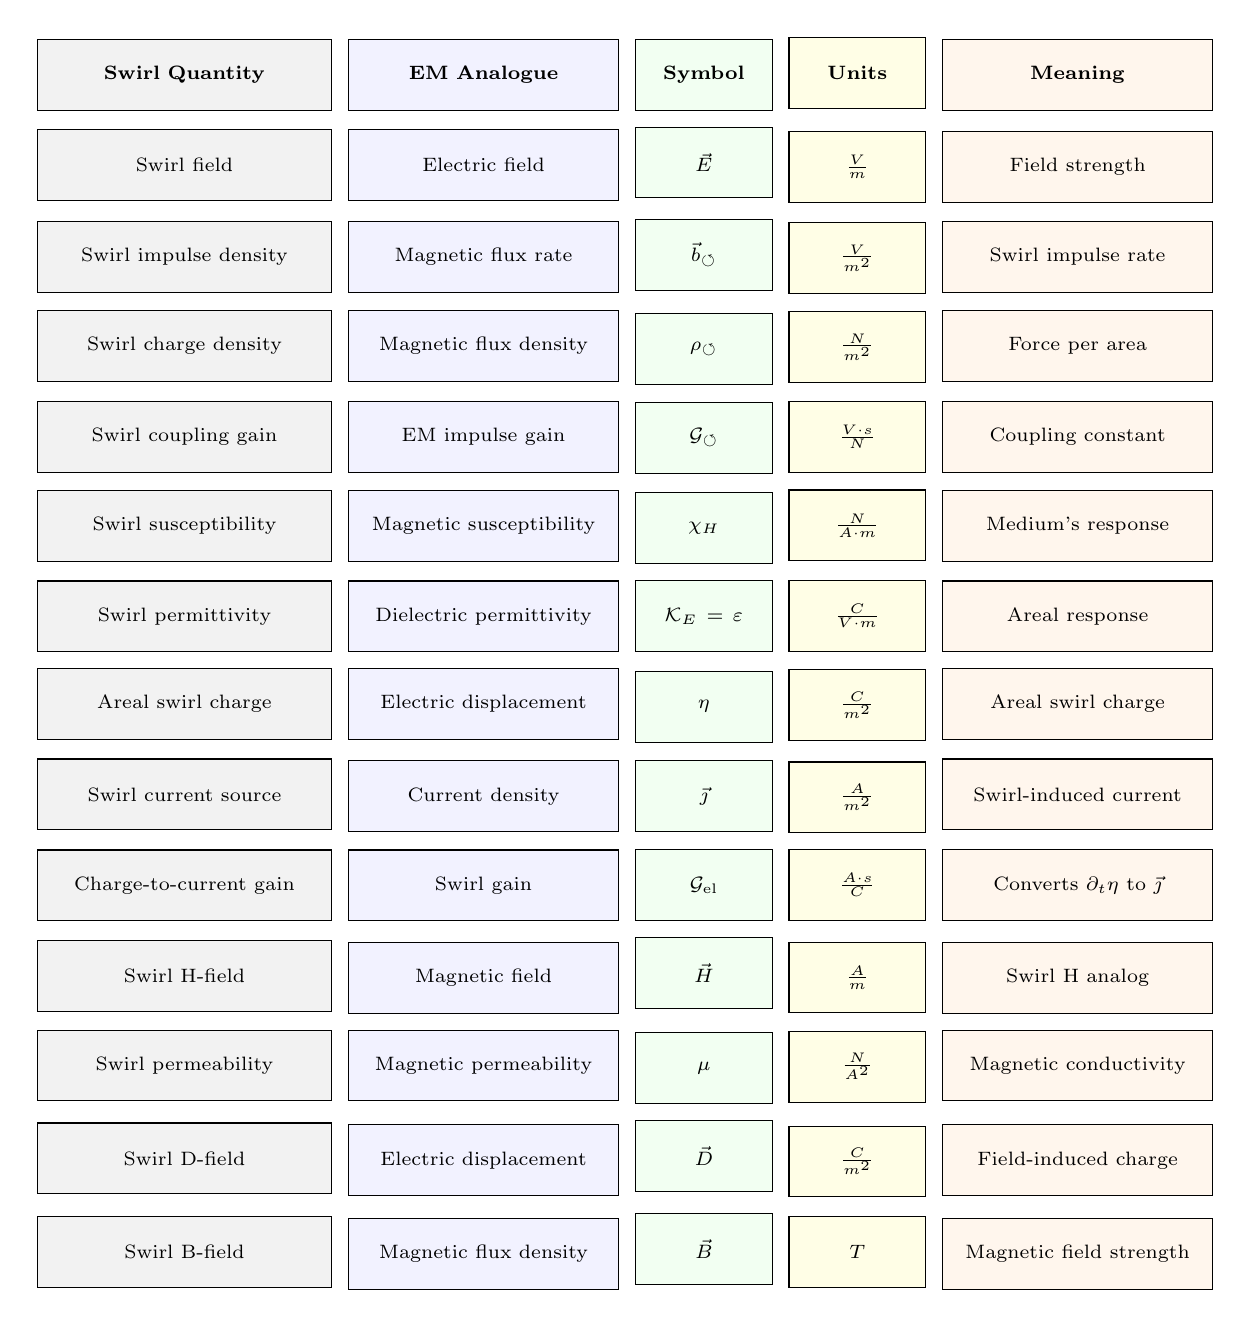
\begin{tikzpicture}
    \tikzset{
        tablecell/.style={
            draw, align=center, font=\scriptsize,
            text height=1.9ex, text depth=.6ex,   % <-- uniform vertical metrics
            inner sep=2pt, minimum height=0.9cm
        }
    }
    \matrix[matrix of nodes,
        nodes={draw, align=center, font=\scriptsize, text width=3.2cm, minimum height=0.9cm},
        column sep=0.2cm, row sep=0.2cm,
        column 1/.style={nodes={text width=3.5cm, fill=gray!10}},
        column 2/.style={nodes={fill=blue!5}},
        column 3/.style={nodes={text width=1.5cm, fill=green!5}},
        column 4/.style={nodes={text width=1.5cm, fill=yellow!10}},
        column 5/.style={nodes={fill=orange!7}}
    ] (m) {
        \textbf{Swirl Quantity} & \textbf{EM Analogue} & \textbf{Symbol} & \textbf{Units} & \textbf{Meaning} \\
        Swirl field & Electric field & $\vec{E}$ & $\tfrac{V}{m}$ & Field strength \\
        Swirl impulse density & Magnetic flux rate & $\vec{b}_{\circlearrowleft}$ & $\tfrac{V}{m^2}$ & Swirl impulse rate \\
        Swirl charge density & Magnetic flux density & $\rho_{\circlearrowleft}$ & $\tfrac{N}{m^2}$ & Force per area \\
        Swirl coupling gain & EM impulse gain & $\mathcal{G}_{\circlearrowleft}$ & $\tfrac{V\cdot s}{N}$ & Coupling constant \\
        Swirl susceptibility & Magnetic susceptibility & $\chi_H$ & $\tfrac{N}{A \cdot m}$ & Medium’s response \\
        Swirl permittivity & Dielectric permittivity & $\mathcal{K}_E = \varepsilon$ & $\tfrac{C}{V \cdot m}$ & Areal response \\
        Areal swirl charge & Electric displacement & $\eta$ & $\tfrac{C}{m^2}$ & Areal swirl charge \\
        Swirl current source & Current density & $\vec{\jmath}$ & $\tfrac{A}{m^2}$ & Swirl-induced current \\
        Charge-to-current gain & Swirl gain & $\mathcal{G}_{\mathrm{el}}$ & $\tfrac{A \cdot s}{C}$ & Converts $\partial_t \eta$ to $\vec{\jmath}$ \\
        Swirl H-field & Magnetic field & $\vec{H}$ & $\tfrac{A}{m}$ & Swirl H analog \\
        Swirl permeability & Magnetic permeability & $\mu$ & $\tfrac{N}{A^2}$ & Magnetic conductivity \\
        Swirl D-field & Electric displacement & $\vec{D}$ & $\tfrac{C}{m^2}$ & Field-induced charge \\
        Swirl B-field & Magnetic flux density & $\vec{B}$ & $T$ & Magnetic field strength \\
    };
    \end{tikzpicture}
    \caption{Canonical Swirl–Electromagnetic Unit Bridge Table}\label{fig:swirl_em_units}
    \end{figure}



\end{document}
